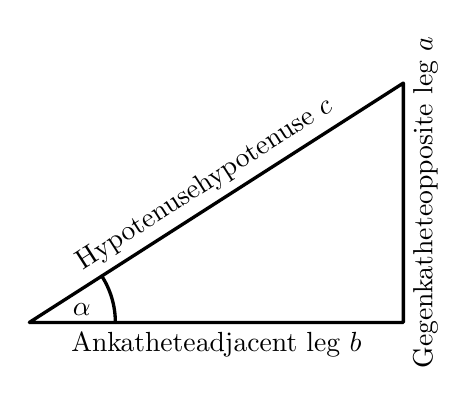
\begin{tikzpicture}[scale=0.95,line cap=round,line join=round]
  \coordinate (A) at (0,0);
  \coordinate (B) at (5,0);
  \coordinate (C) at (5,3.2);

  \draw[very thick] (A) -- (B) -- (C) -- cycle;
  \RightAngleMark{(B)}{90}{180}{0.42}
  \draw[very thick] (1.15,0) arc[start angle=0,end angle=32.6,radius=1.15];

  \node at (0.70,0.17) {$\alpha$};
  \node[below] at (2.5,0) {\Lang{Ankathete}{adjacent leg} $b$};
  \path (B) -- node[midway,sloped,below]
    {\Lang{Gegenkathete}{opposite leg} $a$} (C);
  \path (A) -- node[midway,sloped,above]
    {\Lang{Hypotenuse}{hypotenuse} $c$} (C);
\end{tikzpicture}
